\begin{figure} [h!]
\begin{center}

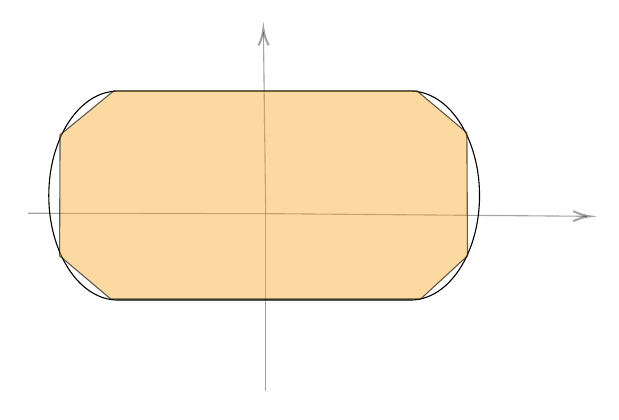
\begin{tikzpicture}[x=0.55pt,y=0.55pt,yscale=-1,xscale=1]
%uncomment if require: \path (0,300); %set diagram left start at 0, and has height of 300

%Straight Lines [id:da10201365463278256] 
\draw [color={rgb, 255:red, 0; green, 0; blue, 0 }  ,draw opacity=0.36 ]   (324,143.5) -- (322.52,24) ;
\draw [shift={(322.5,22)}, rotate = 449.29] [color={rgb, 255:red, 0; green, 0; blue, 0 }  ,draw opacity=0.36 ][line width=0.75]    (10.93,-3.29) .. controls (6.95,-1.4) and (3.31,-0.3) .. (0,0) .. controls (3.31,0.3) and (6.95,1.4) .. (10.93,3.29)   ;
%Straight Lines [id:da6957790210068775] 
\draw [color={rgb, 255:red, 0; green, 0; blue, 0 }  ,draw opacity=0.36 ]   (324,143.5) -- (324,260.25) ;
%Straight Lines [id:da17513960825207286] 
\draw [color={rgb, 255:red, 0; green, 0; blue, 0 }  ,draw opacity=0.36 ]   (168,143.25) -- (324,143.5) ;
%Straight Lines [id:da5820199298694646] 
\draw [color={rgb, 255:red, 0; green, 0; blue, 0 }  ,draw opacity=0.36 ]   (324,143.5) -- (535,145.23) ;
\draw [shift={(537,145.25)}, rotate = 180.47] [color={rgb, 255:red, 0; green, 0; blue, 0 }  ,draw opacity=0.36 ][line width=0.75]    (10.93,-3.29) .. controls (6.95,-1.4) and (3.31,-0.3) .. (0,0) .. controls (3.31,0.3) and (6.95,1.4) .. (10.93,3.29)   ;
%Flowchart: Terminator [id:dp7571888204896569] 
\draw   (226.78,63) -- (419.22,63) .. controls (444.23,63) and (464.5,93.72) .. (464.5,131.63) .. controls (464.5,169.53) and (444.23,200.25) .. (419.22,200.25) -- (226.78,200.25) .. controls (201.77,200.25) and (181.5,169.53) .. (181.5,131.63) .. controls (181.5,93.72) and (201.77,63) .. (226.78,63) -- cycle ;
%Shape: Polygon [id:ds9338072370258934] 
\draw  [color={rgb, 255:red, 0; green, 0; blue, 0 }  ,draw opacity=0.62 ][fill={rgb, 255:red, 245; green, 166; blue, 35 }  ,fill opacity=0.43 ] (224.2,62.8) -- (423.4,62.8) -- (456.2,90.4) -- (456.6,171.2) -- (425.8,199.6) -- (222.2,199.6) -- (188.6,171.2) -- (188.9,91.75) -- cycle ;
\end{tikzpicture}

\end{center} 
% \caption{Visualization of trajectory generation done in the developed software}
\end{figure}